% Created 2018-08-10 Fri 00:05
% Intended LaTeX compiler: pdflatex
\documentclass[presentation, t]{beamer}
\usepackage[utf8]{inputenc}
\usepackage[T1]{fontenc}
\usepackage{graphicx}
\usepackage{grffile}
\usepackage{longtable}
\usepackage{wrapfig}
\usepackage{rotating}
\usepackage[normalem]{ulem}
\usepackage{amsmath}
\usepackage{textcomp}
\usepackage{amssymb}
\usepackage{capt-of}
\usepackage{hyperref}
\setbeamertemplate{navigation symbols}{}
% typeset source code listings
\usepackage{listings}
\usepackage{xcolor}

\definecolor{mc@lstidentifier}{HTML}{000000} % black
\definecolor{mc@lstcomment}{HTML}{008200} % green
\definecolor{mc@lststring}{HTML}{FF5500} % orange
\definecolor{mc@lstkeyword}{HTML}{0000FF} % blue
\definecolor{mc@lstbackground}{HTML}{FFFFCC} % light yellow
\definecolor{mc@lstframe}{HTML}{FFEE88} % dark yellow
\lstdefinelanguage{org}{%
morekeywords={:results, :session, :var, :noweb, :exports},
sensitive=false,
morestring=[b]",
morecomment=[l]{\#},
}
\lstset{%
lineskip=-0.1em,
%
basicstyle=\ttfamily\scriptsize, % font that is used for the code
identifierstyle=\color{mc@lstidentifier},
commentstyle=\color{mc@lstcomment}\itshape,
stringstyle=\color{mc@lststring},
keywordstyle=\color{mc@lstkeyword},
%
extendedchars=true,
inputencoding=utf8,
upquote, %
tabsize=4, % set default tabsize to 4 spaces
showtabs=false, % show tabs within strings adding particular underscores
%  tab=$\to$,
showspaces=false, % show spaces adding particular underscores
showstringspaces=false, % underline spaces within strings
%
numbers=left, % where to put the line numbers
stepnumber=0, % step between two line numbers
numberstyle=\tiny, % line number font size
%
captionpos=b, % set the caption position to `bottom'
%
xleftmargin=0.4em, % text to the right
xrightmargin=0.4em, % text to the left
breaklines=false, % don't break long lines of code
%
frame=single, % add a frame around the code
framexleftmargin=0pt, % frame back to the left
framexrightmargin=0pt, % frame back to the right
backgroundcolor=\color{mc@lstbackground}, % set the background color
rulecolor=\color{mc@lstframe}, % frame color
%
columns=flexible, % try not to ruin the spacing intended by the font designer
keepspaces=true, % don't drop spaces to fix column alignment
%
mathescape, % allow escaping to (La)TeX mode within $..$
% escapechar=², % allow escaping to (La)TeX mode within ²..²
% The backquote was NOT judicious: in some code (comments), I wrap vars
% between such a backquote (`var')
%
% conversion of UTF-8 chars to latin1
literate=
{á}{{\'a}}1
{à}{{\`a}}1
{â}{{\^a}}1
{ä}{{\"a}}1
{ç}{{\c{c}}}1
{é}{{\color{black}\'e}}1
{è}{{\`e}}1
{ê}{{\^e}}1
{ë}{{\"e}}1
{í}{{\'i}}1
{ì}{{\`i}}1
{î}{{\^i}}1
{ï}{{\"i}}1
{ó}{{\'o}}1
{ò}{{\`o}}1
{ô}{{\^o}}1
{ö}{{\"o}}1
{ú}{{\'u}}1
{ù}{{\`u}}1
{û}{{\^u}}1
{ü}{{\"u}}1
{Á}{{\'A}}1
{À}{{\`A}}1
{Â}{{\^A}}1
{Ä}{{\"A}}1
{Ç}{{\c{C}}}1
{É}{{\'E}}1
{È}{{\`E}}1
{Ê}{{\^E}}1
{Ë}{{\"E}}1
{Í}{{\'I}}1
{Ì}{{\`I}}1
{Î}{{\^I}}1
{Ï}{{\"I}}1
{Ó}{{\'O}}1
{Ò}{{\`O}}1
{Ô}{{\^O}}1
{Ö}{{\"O}}1
{Ú}{{\'U}}1
{Ù}{{\`U}}1
{Û}{{\^U}}1
{Ü}{{\"U}}1
}

\definecolor{TeXbackgroundcolor}{HTML}{F1F9EF}
\definecolor{TeXrulecolor}{HTML}{D4E8E3}
\lstdefinestyle{TeX}{backgroundcolor=\color{TeXbackgroundcolor},rulecolor=\color{TeXrulecolor}}
\definecolor{mylinkcolor}{HTML}{006DAF}
\hypersetup{colorlinks=true, linkcolor=mylinkcolor, urlcolor=mylinkcolor}
\usetheme{Madrid}

\author[O. Gutú y J. Waissman]{\href{mailto:olivia.gutu@unison.mx}{Olivia Gutú} y \href{mailto:julio.waissman@unison.mx}{Julio Waissman}}
\date{5 de mayo de 2021}
\title{Modelado de tópicos}
\subtitle{Curso de procesamiento de lenguaje natural}
\institute[MCD]{Maestría en Ciencia de Datos\\ Universidad de Sonora}
\titlegraphic{
\includegraphics[width=0.2\textwidth]{imagenes/MCDLogo.png}}

\usepackage[spanish]{babel}
\usepackage[spanish]{bm}

\hypersetup{
 pdfauthor={\href{mailto:olivia.gutu@unison.mx}{Olivia Gutú} y \href{mailto:julio.waissman@unison.mx}{Julio Waissman}},
 pdftitle={Modelado de tópicos},
 pdfkeywords={},
 pdfsubject={PLN/MCD-UNISON},
 pdflang={Spanish}}
\begin{document}

\maketitle

%--------------------------------------------------------------------

\begin{frame}{¿Que es modelado de tópicos?}
\begin{figure}[htbp]
\centering
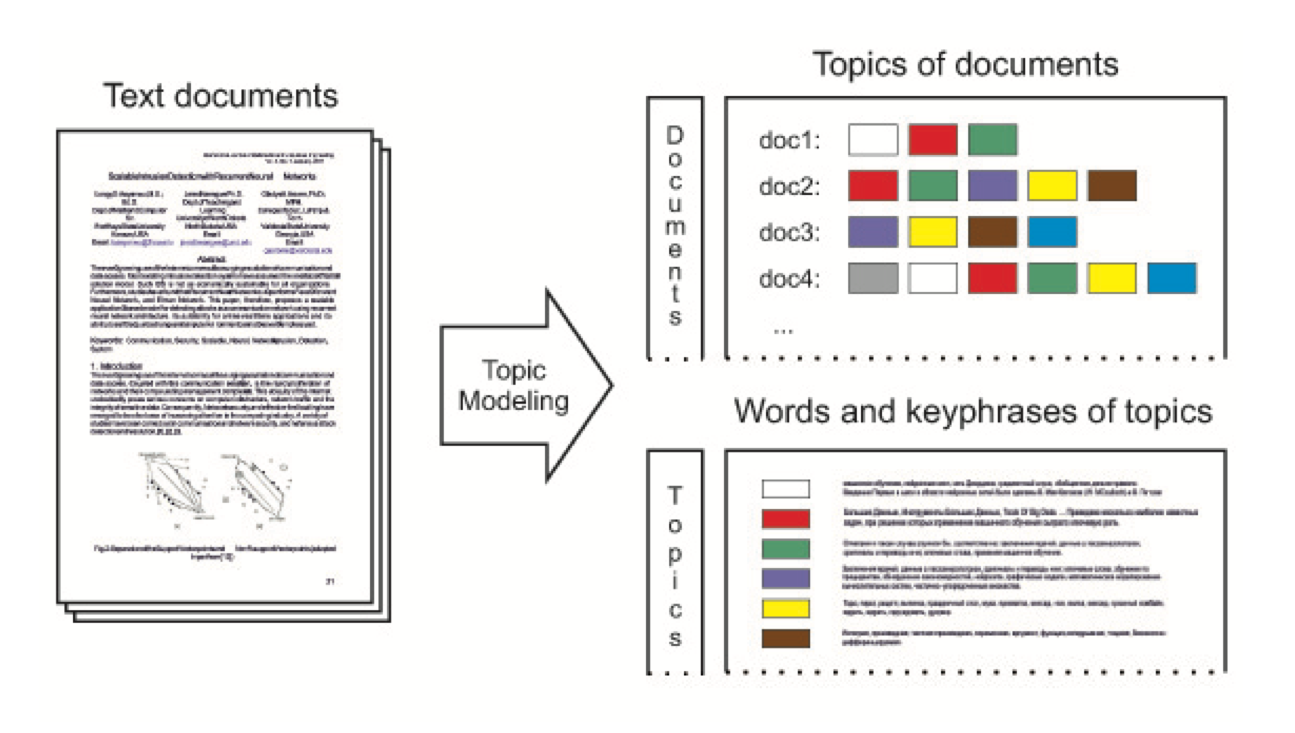
\includegraphics[width=\textwidth]{./imagenes/topic.png}
\end{figure}
\end{frame}

%--------------------------------------------------------------------

\begin{frame}{Definición formal}
\begin{itemize}
\item \alert{Dado}:
\begin{itemize}
\item \(\{d_1, \ldots, d_D\}\) un conjunto de documentos (corpus),
\item \(\{w_1, \ldots, \w_W\}\) un conjunto de palabras (vocabulario),
\item \(n_{dw}\) el número de veces que la palabra \(w\) aparece en el documento \(d\)\vfill
\end{itemize}

\item \alert{Encontrar}:
\begin{itemize}
\item Para un conjunto de \(T\) tópicos \(\{t_1, \ldots, t_T\}\)
\item \(\phi_{wt} = \Pr(w|t)\) una distribución de palabras en cada tópico,
\item \(\theta_{td} = \Pr(t|d)\) una distribución de tópicos por cada documento \vfill
\end{itemize}

\item \alert{Basado en las hipótesis}:
\begin{itemize}
\item Un \emph{tópico} es un conjunto coherente de palabras que co-ocurren en un subconjunto de documentos
\item Un documento está representado con una BOW con cuentas (o proporcional)
\item Toda palabra observada en un documento tiene un \emph{tópico latente}\vfill
\end{itemize}
\end{itemize}
\end{frame}

%--------------------------------------------------------------------

\begin{frame}{¿Para qué sirve el modelado de tópicos?}
\begin{center}
\bf El modelado de tópicos provée una representación semántica
inherente a un conjunto de documentos
\end{center}

Se utiliza en:

\begin{enumerate}
\item Categorización de textos
\item Agregación y resumen de noticias
\item Sistemas de recomendación
\item Recuperación de la información
\item Segmentación de corpus
\end{enumerate}
\end{frame}

%--------------------------------------------------------------------

\begin{frame}{Modelo probabilístico}
\begin{enumerate}
\item Ley de probabilodad total (marginalización)
\[\Pr(w) = \sum_{t \in T} \Pr(w|t)\Pr(t)\]

\item Hipótesis de independencia condicional
\[\Pr(w|t, d) = \Pr(w|t)\]
\end{enumerate}

\begin{block}{Planteamiento}
\[\Pr(w|d) = \sum_{t \in T} \Pr(w|t, d) \Pr(t|d) = \sum_{t \in T} \Pr(w|t)\Pr(t|d) = \phi_{wt}\theta_{td}\]
\end{block}
\end{frame}
\begin{frame}[label={sec:orgae94f4b}]{Visto en forma matricial}
\begin{figure}[htbp]
\centering
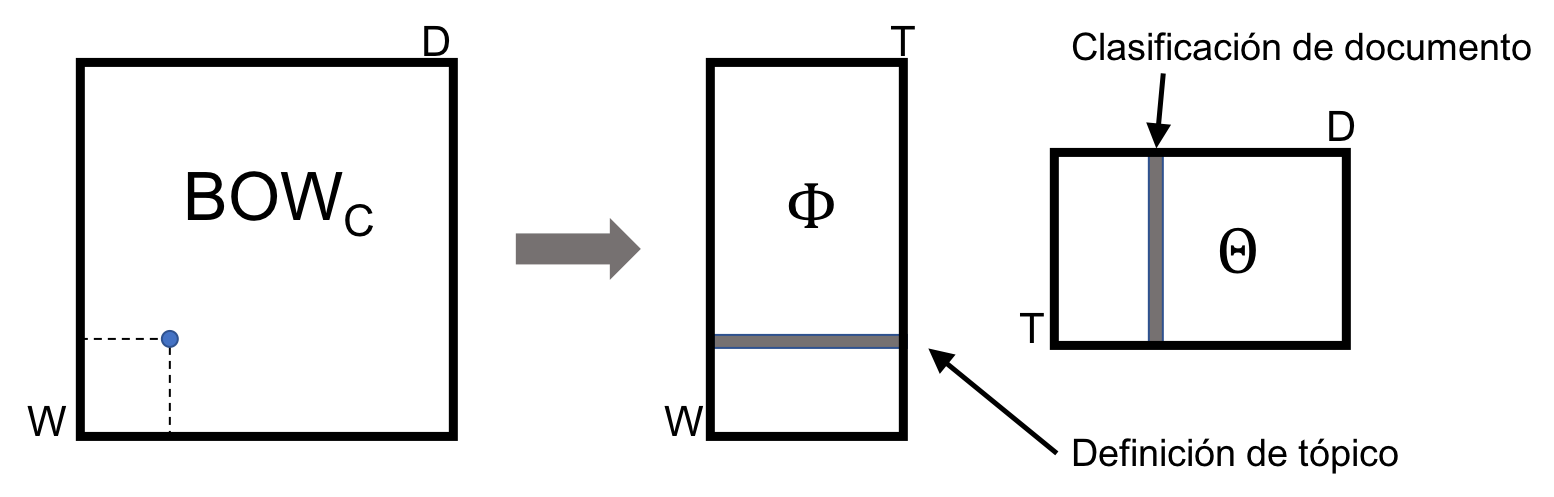
\includegraphics[width=.9\textwidth]{./imagenes/plsa.png}
\end{figure}

\begin{center}
\bf El problema de descomposición matricial en este caso está
pobremente definido, y hay que utilizar algún criterio de optimización
para encontrar las matrices \(\Phi\) y \(\Theta\)
\end{center}
\end{frame}

%--------------------------------------------------------------------

\begin{frame}{PLSA}
\begin{block}{Se optimiza la verosimilitud logarítmica}
\[\Phi^*, \Theta^* = \arg \max_{\Phi, \Theta} \sum_{d} \sum_{w \in
   d} n_{dw} \log \sum_{t}\phi_{wt}\theta_{td}\] \vfill
\end{block}


\begin{center}
\bf Si conociéramos los tópicos sería muy parecido a los vectores de
palabra, pero resulta que solo sabemos el número de tópicos que
imponemos \vfill
\end{center}
\end{frame}

%--------------------------------------------------------------------

\begin{frame}{Algoritmo EM}
\begin{block}{Expectation}
\[\Pr(t|d,w) = \frac{\Pr(w|t)\Pr(t|d)}{\Pr(w|d)} = \frac{\phi_{wt}\theta_{td}}{\sum_{s}\phi_{ws}\theta_{sd}}\]\vfill
\end{block}

\begin{block}{Maximization}
\[\phi_{wt} = \frac{n_{wt}}{\sum_{v}n_{vt}} \quad \text{donde} \quad n_{wt} = \sum_{d}n_{dw}\Pr(t|d,w)\]
\[\theta_{td} = \frac{n_{td}}{\sum_{t'}n_{t'd}} \quad \text{donde} \quad n_{td} = \sum_{w}n_{dw}\Pr(t|d,w)\]\vfill
\end{block}
\end{frame}

%--------------------------------------------------------------------

\begin{frame}{Latent Dirichlet Allocation (LDA)}
\begin{figure}[htbp]
\centering
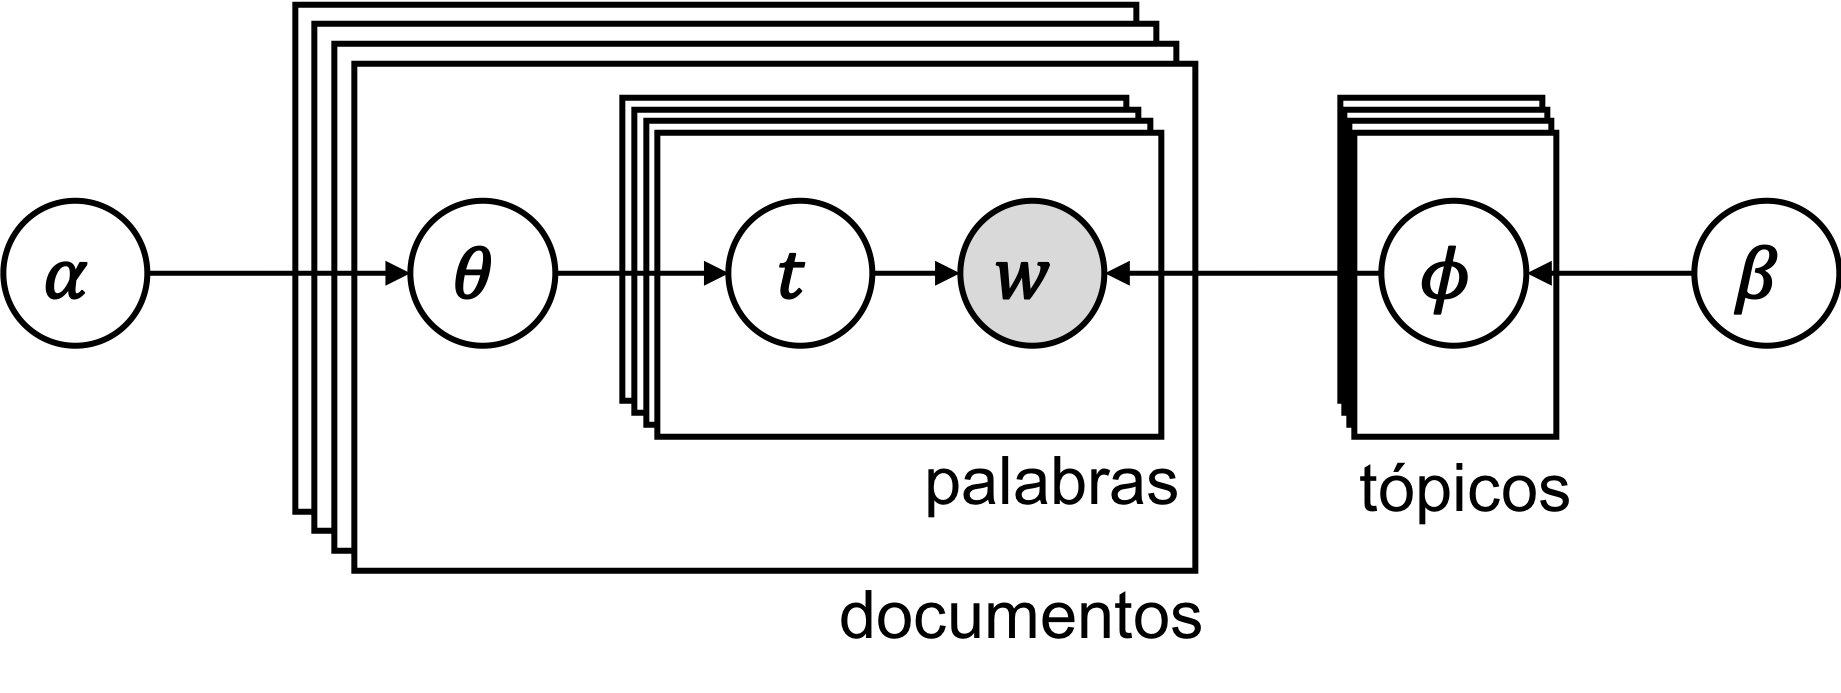
\includegraphics[width=.75\textwidth]{./imagenes/lda.png}
\end{figure}

\begin{enumerate}
\item La distribución de palabras para el tópico \(t\) (\(\phi_t\), el \(t\)-ésimo un renglón de \(\Phi\)) es
generada por una distribución de \emph{Dirichlet} con parámetros \(\beta \in \mathbb{R}^W\)

\item La distribución de tópicos para el documento \(d\) (\(\theta_d\) una columna de \(\Theta\)) también se genera a partir
de una distribución de \emph{Dirichlet} con parámetros \(\alpha \in \mathbb{R}^T\)
\end{enumerate}
\end{frame}

%--------------------------------------------------------------------


\begin{frame}{Modelado de tópicos multimodal}
\begin{figure}[htbp]
\centering
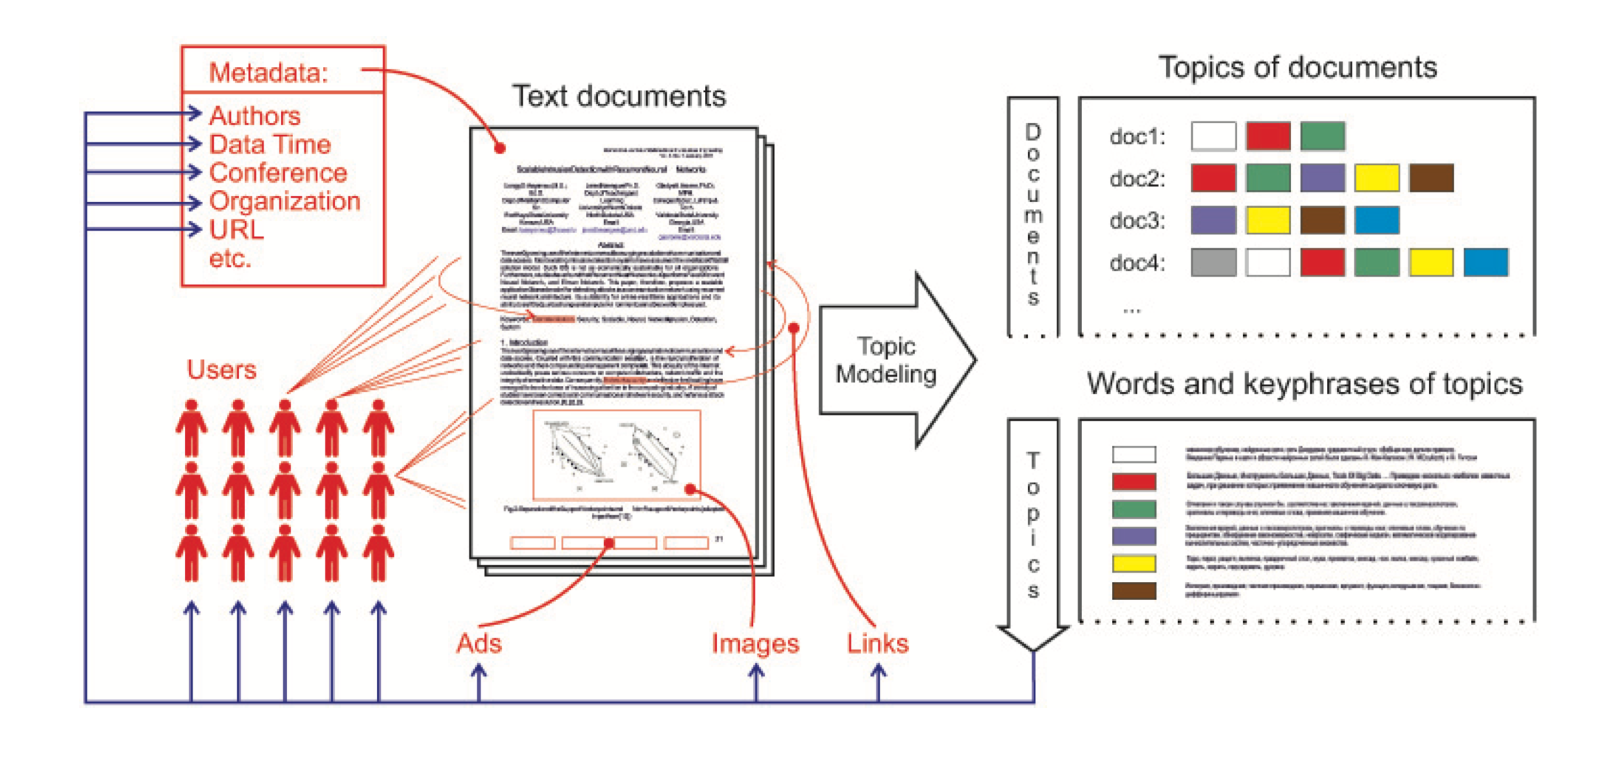
\includegraphics[width=.85\textwidth]{./imagenes/mmtm.png}
\end{figure}
\begin{center}
Biblioteca especializada \emph{BigARTM} en \href{http://bigartm.org}{http://bigartm.org}
\end{center}
\end{frame}

%--------------------------------------------------------------------

\begin{frame}{Revisemos el modelado de tópicos}
\begin{figure}[htbp]
\centering

\includegraphics[width=.35\textwidth]{./imagenes/jupyter.png}
\end{figure}
\begin{center}
   Ejemplo con los sonetos del siglo de oro español

   \href{https://github.com/juliowaissman/lda-ejemplo}{https://github.com/juliowaissman/lda-ejemplo}
\end{center}
\end{frame}
%--------------------------------------------------------------------

\end{document}